%======================================================================================== 
%Preamble. Latex needs all this stuff to work, but it doesn't appear in your document.
\documentclass{article}[12pt]
\usepackage{geometry}                
\usepackage{graphicx}
\usepackage{amsmath}
\usepackage{amssymb}
\usepackage{float}
\floatstyle{plain}
\usepackage[]{microtype}
\usepackage{listings}
\lstset{
    literate={~} {$\sim$}{1}
}
\usepackage{color}
\usepackage{epstopdf}

\usepackage{lipsum}
\newcommand{\eqname}[1]{\tag*{\bf #1}}% Tag equation with name
%\DeclareGraphicsRule{.tif}{png}{.png}{`convert #1 `dirname #1`/`basename #1 .tif`.png}
\usepackage{hyperref}
\hypersetup{
    colorlinks=true,
    linkcolor=blue,
    filecolor=magenta,      
    urlcolor=blue,
    citecolor={blue}
    }
    
\usepackage[backend=biber, style=authoryear, uniquename=false,doi=false,isbn=false, url=false, giveninits]{biblatex}
\usepackage[utf8]{inputenc}
\usepackage[toc, section=section]{glossaries}
\addbibresource{FYP_references.bib}


\makeglossaries
\newglossaryentry{CNCC}
    {name = CNCC,
    description = {Cranial Neural Crest Cell}
}
\newglossaryentry{EPO}
    {name = EPO,
    description = {Enredo, Pecan, Ortheus pipeline algorithm used by Ensembl to construct a multiple sequence alignment from sequences generated from pairwise whole-genome alignments}
}
\newglossaryentry{FOXC1}
    {name = FOXC1,
    description = {Forkhead Box C1 Gene}
}
\newglossaryentry{GRN}
    {name = GRN,
    description = {Genetic Regulatory Network}
}
\newglossaryentry{GTR}
    {name = GTR,
    description = {General Time-Reversible model of nucleotide substitution}
}
\newglossaryentry{HAR}
    {name = HAR,
    description = {Human-Accelerated Region}
}
\newglossaryentry{LRT}
    {name = LRT,
    description = {Likelihood Ratio Test}
}
\newglossaryentry{MSA}
    {name = MSA,
    description = {Multiple Sequence Alignment}
}
\newglossaryentry{NCC}
    {name = NCC,
    description = {Neural Crest Cell}
}
\newglossaryentry{SSREV}
    {name = SSREV,
    description = {Strand-symmetric time-reversible model of nucleotide substitution}
}

%\usepackage{biblatex}
%==========================================================
% My title, name, and date
\title{FOXC1 \emph{cis}-regulatory region shows accelerated evolution in \emph{Homo sapiens}}
\author{Esta V. Shrewsbury}
%==========================================================

\setlength{\parskip}{1em}

\begin{document}

\maketitle

\section{Abstract}

Research has shown that the \Gls{CNCC} pathway is largely responsible for craniofacial variation in amniotes. This pathway is highly conserved and plays a key role in determining many anatomical \& physiological phenotypes during amniote development. Geometric morphometric studies of primate skulls show that human jaws have undergone accelerated evolution following our divergence from chimpanzees, this suggests there are genes or sequences linked to the CNCC pathway that also show accelerated evolution in the human genome. The aim of this project was to test for acceleration in the \emph{cis}-regulatory enhancer of the \Gls{FOXC1} gene. This sequence was selected from a comparative gene expression study which found evidence of human-biased FOXC1 expression in human CNCC cultures (in comparison to chimpanzee CNCC cultures). A meta-analysis was carried out on an \Gls{MSA} for this 200 base-pair regulatory sequence and 23 homologous primate sequences. The results of this analysis showed no significant evidence for evolutionary conservation in this aligned sequence for non-human primates, but a few coordinates of the human sequence showed accelerated evolution. Further analysis may help to build a better understanding of the genetic basis behind the accelerated rate of evolution in human jaw development.
\newpage

\tableofcontents
\printglossary

\newpage

\section{Introduction}

Humans show many uniquely derived anatomical and behavioural features that make us stand out from other primates. Unlike other apes, humans have flatter faces with a characteristic round skull shape, less-pronounced brow ridges and significantly reduced prognathism \parencite{Martinez2009}. Geometric morphometric analyses on primate skulls have highlighted these features as the key components of our craniofacial anatomy that show the greatest variation between humans and other primates \parencite{Raia2018}. This study has also shown that human jaws have undergone an accelerated rate of evolution following our divergence from chimpanzees.

The genetic basis for interspecific craniofacial differences is still poorly understood as the genetic pathways responsible are complex and highly conserved – this includes the \Gls{CNCC} pathway. Since humans share over 95\% of our DNA with chimpanzees \parencite{Suntsova2020}, this limits our search down to the remaining divergent ~5\% of the genome that must explain all of the phenotypical differences between humans and chimpanzees. The majority of these varied sequences are pleiotropic regulatory genes \parencite{Franchini2017}.

The \Gls{NCC} pathway is a \Gls{GRN} that controls the induction and migration of the NCC population at key points during vertebrate embryogenesis. NCCs are a temporary group of multipotent stem cells that can differentiate into many diverse cell lineages, the Neural Crest is established following induction via the BMP, Wnt and FGF cell signalling pathways. This activates expression of various transcription factors, such as \emph{Snail}/\emph{Slug}, \emph{Foxd3} \& \emph{SoxE}, which subsequently the borders of the NCC populations that act as precursors to various tissues – e.g., the mesenchyme differentiates into osteoblasts (bone), myocytes (muscle), and chondroblasts (cartilage) etc. \parencite{Huang2004, Kulesa2010}

Depending on their position along the anterior-posterior axis of the developing organism during NCC induction, the cell lineages will follow one of four different functional pathways. These are the cranial, trunk, vagal \& sacral, or the cardiac neural crest. The CNCCs will migrate in a species-specific pattern along the dorso-lateral axis of the head thus determining the craniofacial mesenchyme \parencite{Kulesa2010}.

Genetic studies focused on human evolution have coined the term Human Accelerated Regions (HARs) applying to sequences within the human genome that are conserved in vertebrates but show significant nucleotide divergence in humans \parencite{Gittelman2015}. These regions were identified through comparative analyses between human and chimpanzee genomes. This study tests for these \Gls{HAR} requirements in a multiple sequence alignment of the \emph{cis}-regulatory sequence the FOXC1 gene, although I focused specifically on primates.

This gene was identified in a comparative study between cultured human \& chimpanzee CNCCs and their respective gene expression profiles \parencite{Prescott2015}. This study showed that FOXC1, along with multiple other genes linked to the CNCC pathway, showed significantly higher expression in human CNCCs than in chimpanzee CNCC – described as human-biased activity. The increased expression of FOXC1 in human CNCC was subsequently linked to a \emph{cis}-regulatory enhancer sequence located downstream from FOXC1 in the human chromosome 6.

\emph{Cis}-regulatory elements are non-coding regions of the genome that regulate the expression of neighbouring by acting as binding sites for transcription factors, this promotes the transcription of the associated gene. 

The initial hypothesis was CNCC pathway associated genes that showed species-biased activity in humans or chimpanzees will have \emph{cis}-regulatory enhancers that may show evidence for accelerated evolution when compared to homologous sequences in primates. This could partially explain the genetic basis for accelerated evolution in human jaw development. 


%Figure 1
\floatstyle{plain}
\restylefloat{figure}
\begin{figure}[H]
\centering
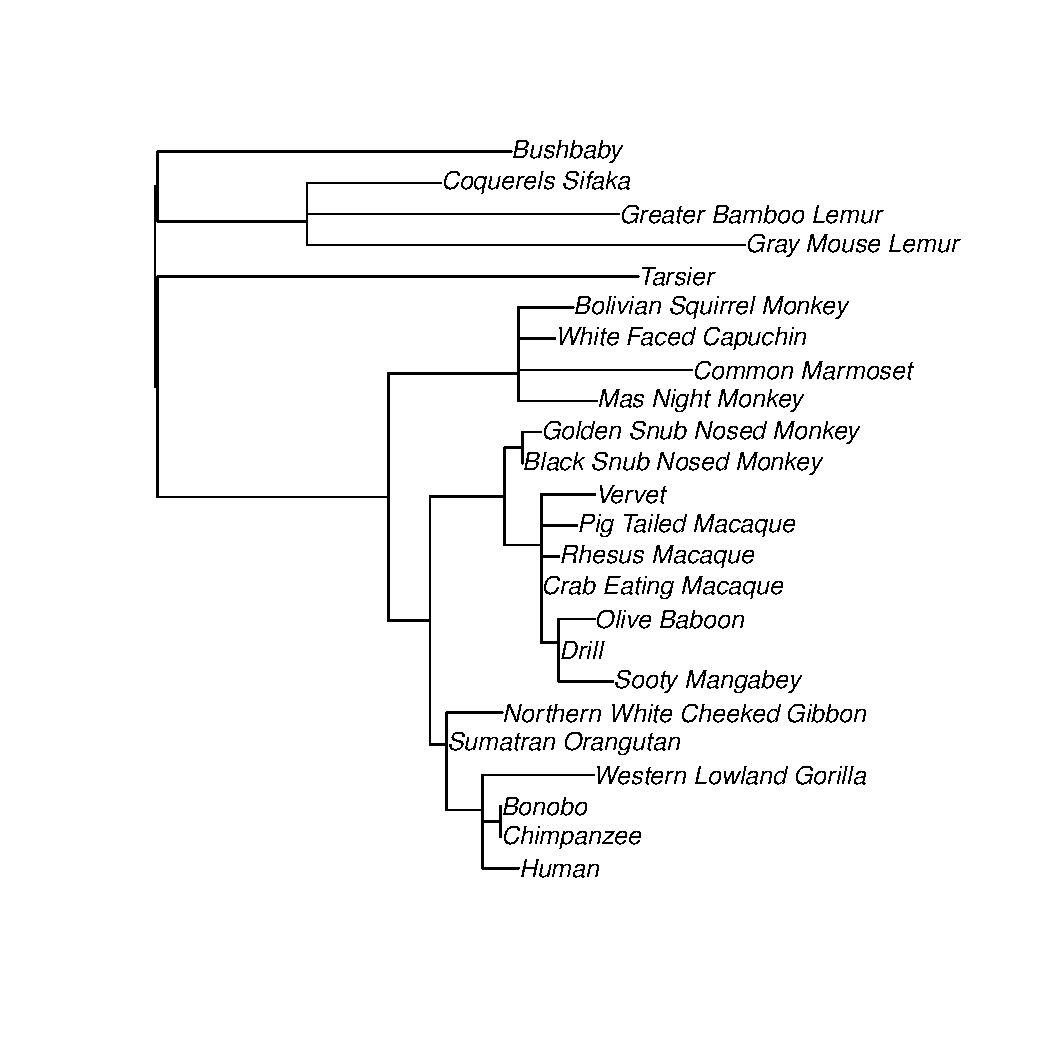
\includegraphics[width=12cm]{neutral_tree.pdf}
\caption{Phylogenetic tree of 24 primate \Gls{EPO}-alignment of the FOXC1 \emph{cis}-regulatory enhancer sequence. Constructed using the neutral model (phyloFit - estimating branch lengths) and the R package ape \parencite{Ape}}
\label{fig1}
\end{figure}

%Figure 2
\floatstyle{plain}
\restylefloat{figure}
\begin{figure}[H]
\centering
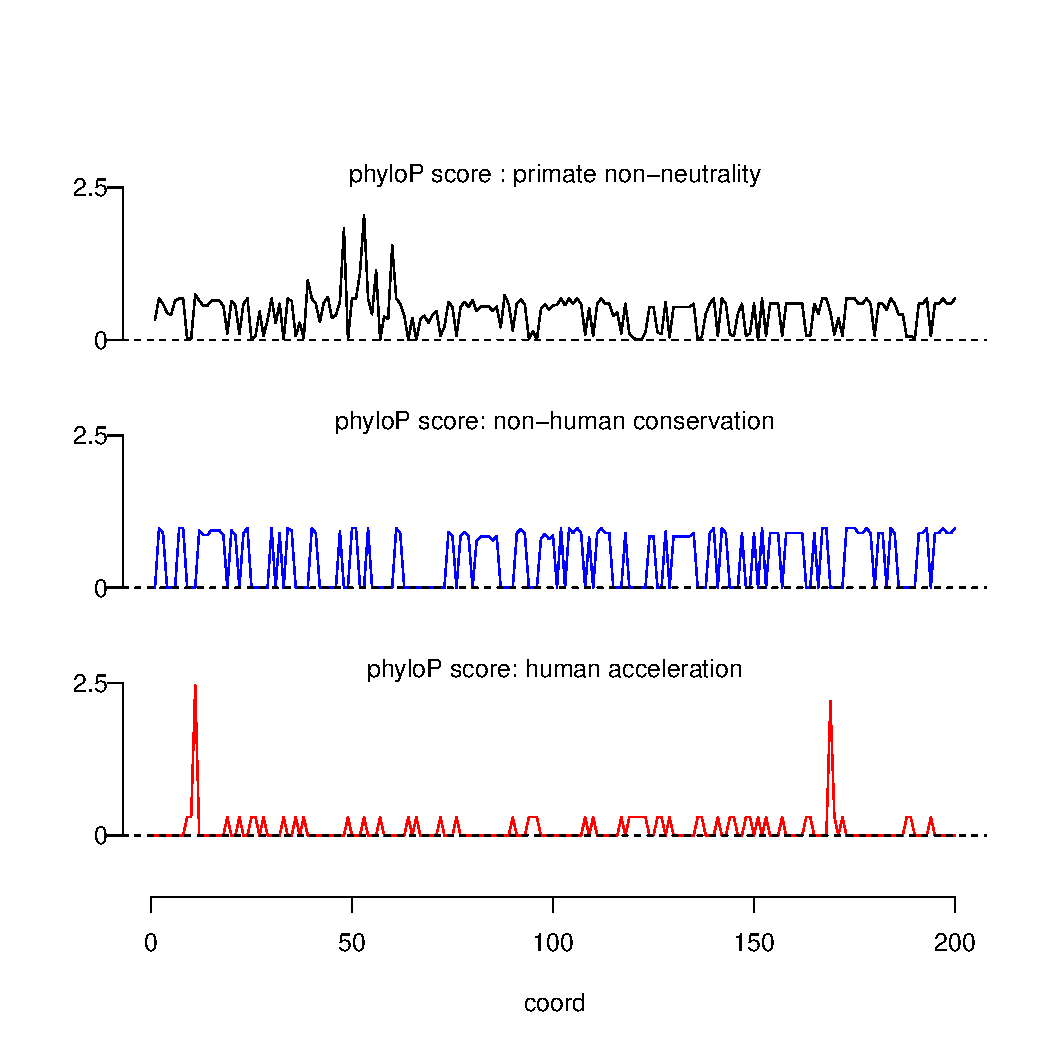
\includegraphics[width=12cm]{compare_phyloP.pdf}
\caption{Plot of phyloP scores for NNEUT, CON and ACC tests described in Methods. This graph was made using the plot.track function provided by the rphast package \parencite{Rphast}}
\label{fig2}
\end{figure}


\section{Methods}

Genomic transcripts for the chosen sequence (chr6: 1744897 – 1745096) were obtained using the Ensembl genomic database \parencite{Ensembl}. An \Gls{MSA} was constructed with Ensembl, containing the initial 200bp human sequence and 23 non-human primate homologs (as predicted by the \Gls{EPO} alignment algorithm automated by the Ensembl database). Ensembl release 104 introduces gaps using the EPO pipeline therefore the MSA was 236bp long although each individual primate sequence ranged around 200bp (coordinates for the comparative regions can be viewed in supplementary material). The EPO-alignment and the representative phylogenetic tree were downloaded in FASTA \& Newick formats, respectively.

Twelve of the total 24 primates selected for the alignment were noted as having low-quality alignment assembly (listed: Sooty Mangabey, Drill, Pig-Tailed Macaque, Black Snub-Nosed Monkey, Golden Snub-Nosed Monkey, Ma’s Night Monkey, White Faced Capuchin, Bolivian Squirrel Monkey, Tarsier, Greater Bamboo Lemur, Coquerel’s Sifaka \& Bushbaby) – this may impact the repeatability of this study.

MSA analysis was carried out using the software R \parencite{R} and the packages Biostrings \parencite{Biostrings}, rphast \parencite{Rphast} \& ape \parencite{Ape}. The rphast package was the key component for this analysis as it allowed us to test for the likelihood of conservation or acceleration within an MSA using phyloP tests.

The phyloP tests require a neutral model of evolution as the null hypothesis. Therefore, we ran a phyloFit test for the MSA to set this model (object class: tm). The parameters set for this were nrates = 4, model = SSREV, EM = TRUE [ref]. Here we used the phylogenetic tree provided with the Ensembl EPO-primate alignment in Newick format to set the neutral tree model (see Figure \ref{fig1}).

The \Gls{SSREV} model is a variant of the \Gls{GTR} model of nucleotide substitution. The SSREV model, in contrast, takes into account the limitations of double-stranded DNA thus the base frequency on one strand changing will directly affect the complementary base frequency on the opposite strand. This model only requires four substitution rate categories (nrates) whereas the normal GTR model requires six \parencite{PhyloP, Gittelman2015}. The neutral model set by phyloFit assumes no selection therefore all nucleotide variation should be sufficiently explained by neutral genetic drift.

Three consecutive phyloP tests were carried out, each outputs a matrix of p-values and scores according to the specified mode. These correspond to the coordinates in the MSA and determine the likelihood of the apparent nucleotide variation fitting the neutral model (previously set with phyloFit) – here the critical value is p-value < 0.05. All three tests used the \Gls{LRT} scoring method - this adds a column for Lnl ratio, which is the ratio of likelihood scores between the two models (i.e., the neutral and the alternative model – mode options: NNEUT, CON, ACC). The Lnl ratio and associated p-values are combined into a score column as plotted in figure 2 (see supplementary data for data matrices of phyloP test results).

The first test included the full primate alignment and the previously constructed neutral model (phyloFit). Here we set the mode parameter to non-neutrality (NNEUT) to test for significant deviation at every coordinate in the alignment from the neutral model – this consequently suggests that the assumption of no selection has been violated, although this could be either evidence for conservation or acceleration in the NNEUT test.

The second phyloP test was run for a subset of the MSA excluding humans. This phyloP test uses the mode conservation (CON). The alternative hypothesis for this test assumes that the 23 primates in this alignment show significantly less nucleotide variation between species than is expected in the neutral alignment – this could suggest negative/purifying selection to decrease nucleotide variation.

The third and final phyloP test used the full alignment, the mode acceleration (ACC) and the parameter subtree = humans. Significant p-values for this test may indicate positive/directional selection due to the introduction of a selective pressure in our recent evolutionary history.


\section{Results}

Three coordinates for the entire primate alignment showed significant p-values for the NNEUT phyloP test. This indicates the nucleotide variation observed at those coordinates (for all primates in this alignment) could not be sufficiently explained by the neutral model. Interestingly, the non-neutral coordinates were located within approximately 20bp of each other – my initial thoughts were that this region could be functionally important, i.e., as a binding site, but further testing is required to explore this hypothesis. (Figure \ref{fig2})

The phyloP test for conservation in the non-human primate subset did not show any significantly conserved coordinates in the sequence. This is one of the requirements for a defined \Gls{HAR} therefore this confirms that this 200bp \emph{cis}-regulatory sequence is not unique to humans and may have undergone rapid evolution in other branches of the primate family tree – as suggested by the NNEUT results.

The phyloP test for human-specific acceleration showed significant p-values at two coordinates located at either end of the sequence. These positions do not overlap with the non-neutral coordinates identified in the full primate phyloP test (NNEUT). 

The results of these tests suggest that this \emph{cis}-regulatory sequence is not unique to humans as a target of evolution as it does not fulfil the conservation requirements of a \Gls{HAR}. This implies that this sequence may be involved in interspecific craniofacial variation for other primate species, we could identify these branches by carrying out further phyloP testing for different subtrees of the primate alignment. Since human-accelerated coordinates of the sequence did not show any significant non-neutrality in first phyloP test, it is likely that those coordinates are not accelerated in any other primates and, by extension, the coordinates of non-neutrality are consistent for multiple species in the alignment.

Since I only analysed an \Gls{MSA} for a single reference sequence, the results for each phyloP test were calculated for each base-pair rather than for extended sequences so there is a definite risk of exaggerating the importance of the test results for specific coordinates. For example, we have made the assumption for this non-coding sequence that the impact of nucleotide variation on functionality (i.e., as a binding site) is the same across the entire sequence when it is possible that mutations at some coordinates are silent and thus may be misinterpreted as non-neutral or accelerated in phyloP tests. This highlights the limitations of a meta-analysis such as this, expression data is often unavailable for less well-known (and therefore less studied) genes which, unfortunately, includes many genes involved in \Gls{CNCC} pathway. Invasive gene expression studies on developing human embryos are obviously highly unethical so the process of mapping out complex \Glspl{GRN} (such as the CNCC pathway) in human and chimpanzee development to their corresponding phenotypes is incredibly difficult. 

Therefore, this meta-analysis attempts to bypass this gap in our understanding of FOXC1’s involvement in human jaw development but, consequently, this means I cannot realistically prove that our chosen regulatory sequence explains the accelerated rate of evolution in human jaws.

As indicated by \cite{Prescott2015}, there are many regulatory sequences linked to CNCC genes that vary between humans and chimpanzees so a useful extension of this study would be to concatenate a selection of these sequences in a single MSA and carry out similar analyses. This concatenated MSA would string multiple different regions for the same species onto one large alignment, subsequent phyloP tests could be altered to output p-values corresponding to an entire sequence rather than for individual bases thus allowing one to candidate sequences for further analysis. This, however, has the disadvantage of losing the level of detail seen in our base-wise phyloP tests.


\section{Discussion}

I've left the discussion out deliberately as I'm still editing it but I promise it exists.

\newpage

\addcontentsline{toc}{section}{References}
\section*{}
\printbibliography

\section{Supplementary Material}


\end{document}